%  LaTeX support: latex@mdpi.com 
%  In case you need support, please attach all files that are necessary for compiling as well as the log file, and specify the details of your LaTeX setup (which operating system and LaTeX version / tools you are using).

%=================================================================
\documentclass[applsci,article,submit,moreauthors,pdftex]{Definitions/mdpi} 

%=================================================================
\firstpage{1} 
\makeatletter 
\setcounter{page}{\@firstpage} 
\makeatother
\pubvolume{xx}
\issuenum{1}
\articlenumber{5}
\pubyear{2020}
\copyrightyear{2020}
%\externaleditor{Academic Editor: name}
\history{Received: date; Accepted: date; Published: date}
%\updates{yes} % If there is an update available, un-comment this line

%% MDPI internal command: uncomment if new journal that already uses continuous page numbers 
%\continuouspages{yes}

%------------------------------------------------------------------
% The following line should be uncommented if the LaTeX file is uploaded to arXiv.org
%\pdfoutput=1

%=================================================================
% Add packages and commands here. The following packages are loaded in our class file: fontenc, inputenc, calc, indentfirst, fancyhdr, graphicx,epstopdf, lastpage, ifthen, lineno, float, amsmath, setspace, enumitem, mathpazo, booktabs, titlesec, etoolbox, tabto, xcolor, soul, multirow, microtype, tikz, totcount, amsthm, hyphenat, natbib, hyperref, footmisc, url, geometry, newfloat, caption

%=================================================================
%% Please use the following mathematics environments: Theorem, Lemma, Corollary, Proposition, Characterization, Property, Problem, Example, ExamplesandDefinitions, Hypothesis, Remark, Definition, Notation, Assumption
%% For proofs, please use the proof environment (the amsthm package is loaded by the MDPI class).

%=================================================================
% Full title of the paper (Capitalized)
\Title{Sound Source Localization Using Graph Regularized Neural Network}

% Author Orchid ID: enter ID or remove command
\newcommand{\orcidauthorA}{0000-0000-000-000X} % Add \orcidA{} behind the author's name
%\newcommand{\orcidauthorB}{0000-0000-000-000X} % Add \orcidB{} behind the author's name

% Author homepage: enter homapage URL or remove command
\newcommand{\homepageauthorA}{https://www.mdpi.com/} % Add \homepageA{} behind the author's name
%\newcommand{\homepageauthorB}{https://www.mdpi.com/} % Add \homepageB{} behind the author's name

% Authors, for the paper (add full first names)
\Author{Firstname Lastname $^{1,\dagger,\ddagger}$\orcidA{}\homepageA{}, Firstname Lastname $^{1,\ddagger}$ and Firstname Lastname $^{2,}$*}

% Authors, for metadata in PDF
\AuthorNames{Firstname Lastname, Firstname Lastname and Firstname Lastname}

% Affiliations / Addresses (Add [1] after \address if there is only one affiliation.)
\address{%
$^{1}$ \quad Affiliation 1; e-mail@e-mail.com\\
$^{2}$ \quad Affiliation 2; e-mail@e-mail.com}

% Contact information of the corresponding author
\corres{Correspondence: e-mail@e-mail.com; Tel.: (optional; include country code; if there are multiple corresponding authors, add author initials) +xx-xxxx-xxx-xxxx (F.L.)}

% Current address and/or shared authorship
\firstnote{Current address: Affiliation 3} 
\secondnote{These authors contributed equally to this work.}
% The commands \thirdnote{} till \eighthnote{} are available for further notes

%\simplesumm{} % Simple summary

%\conference{} % An extended version of a conference paper

% Abstract (Do not insert blank lines, i.e. \\) 
\abstract{A single paragraph of about 200 words maximum. For research articles, abstracts should give a pertinent overview of the work. We strongly encourage authors to use the following style of structured abstracts, but without headings: (1) Background: Place the question addressed in a broad context and highlight the purpose of the study; (2) Methods: Describe briefly the main methods or treatments applied; (3) Results: Summarize the article's main findings; and (4) Conclusion: Indicate the main conclusions or interpretations. The abstract should be an objective representation of the article, it must not contain results which are not presented and substantiated in the main text and should not exaggerate the main conclusions.}

% Keywords
\keyword{keyword 1; keyword 2; keyword 3 (list three to ten pertinent keywords specific to the article, yet reasonably common within the subject discipline.)}

% The fields PACS, MSC, and JEL may be left empty or commented out if not applicable
%\PACS{J0101}
%\MSC{}
%\JEL{}

%%%%%%%%%%%%%%%%%%%%%%%%%%%%%%%%%%%%%%%%%%
% Only for the journal Diversity
%\LSID{\url{http://}}

%%%%%%%%%%%%%%%%%%%%%%%%%%%%%%%%%%%%%%%%%%
% Only for the journal Applied Sciences:
%\featuredapplication{Authors are encouraged to provide a concise description of the specific application or a potential application of the work. This section is not mandatory.}
%%%%%%%%%%%%%%%%%%%%%%%%%%%%%%%%%%%%%%%%%%

%%%%%%%%%%%%%%%%%%%%%%%%%%%%%%%%%%%%%%%%%%
% Only for the journal Data:
%\dataset{DOI number or link to the deposited data set in cases where the data set is published or set to be published separately. If the data set is submitted and will be published as a supplement to this paper in the journal Data, this field will be filled by the editors of the journal. In this case, please make sure to submit the data set as a supplement when entering your manuscript into our manuscript editorial system.}

%\datasetlicense{license under which the data set is made available (CC0, CC-BY, CC-BY-SA, CC-BY-NC, etc.)}

%%%%%%%%%%%%%%%%%%%%%%%%%%%%%%%%%%%%%%%%%%
% Only for the journal Toxins
%\keycontribution{The breakthroughs or highlights of the manuscript. Authors can write one or two sentences to describe the most important part of the paper.}

%\setcounter{secnumdepth}{4}
%%%%%%%%%%%%%%%%%%%%%%%%%%%%%%%%%%%%%%%%%%
\def\apriori{\textit{a priori}}
\usepackage{siunitx}
\usepackage{changebar}
\setlength{\changebarwidth}{2pt}
\cbcolor{red}
\usepackage{booktabs}
\usepackage{todonotes}
\setlength{\marginparwidth}{3cm}
\usepackage[most]{tcolorbox}
\usepackage{graphicx}
\definecolor{block-gray}{gray}{0.85}
\definecolor{MLA2020}{rgb}{1.0,  0.0,  0.5}
\definecolor{JAES2020}{rgb}{0.5,  1.0,  0.5}
\definecolor{JASMP2020}{rgb}{0.75, 1.0,  0.5}
\definecolor{block-C}{rgb}{1.0,  1.0,  0.5}
\definecolor{block-D}{rgb}{1.0,  0.75, 0.5}
\definecolor{block-E}{rgb}{1.0,  0.5,  0.5}
\tcbset{before upper={\parindent0em}}
\newtcolorbox{myquote}{enhanced,colback=block-gray,grow to right by=-10mm,grow to left by=-10mm,
	boxrule=0pt,boxsep=0pt,breakable,arc=3mm}

\newtcolorbox{colquote}[1]{enhanced,colback=#1,grow to right by=0mm,grow to left by=0mm,
	boxrule=0pt,boxsep=0pt,breakable,arc=0mm}

\usepackage[framemethod=tikz]{mdframed}
\mdfsetup{hidealllines=true,innerleftmargin=3pt,innerrightmargin=3pt,leftmargin=-3pt,rightmargin=-3pt}
\def\papertitile{Convolutional Neural Network for Multiple Sound Source Localization in Reverberant Environment}

\usepackage{nth}


\def\doa{\ensuremath{\text{DoA}}}
\def\resdoa{\ensuremath{R_{\doa{}}}}
\def\tdoa{\ensuremath{\text{TDoA}}}
\def\cnn{\ensuremath{\text{CNN}}}
\def\ccfb{\ensuremath{\text{CCFB}}}
\def\pra{\texttt{pyroomaoustics}}
\def\keras{\textit{Keras}}
\def\python{\textit{Python}}
\def\convwe{CONV-WE-CCFB}
\def\convour{CONV-CCFB-DOA}
\def\lr{\ensuremath{\mathrm{lr}}}
\def\az{\ensuremath{\theta}}
\def\el{\ensuremath{\phi}}
\def\relu{ReLU}
\def\framesizeval{\ensuremath{P}}
\def\freqbandnval{\ensuremath{K}}
\def\micpos{\ensuremath{\mathbf{m}}}
\def\srcpos{\ensuremath{\mathbf{s}}}
\def\mic{\ensuremath{{m}}}
\def\src{\ensuremath{{s}}}
\def\micidxi{\ensuremath{i}}
\def\micidxj{\ensuremath{j}}
\def\srcidx{\ensuremath{p}}

\def\roomDim{\ensuremath{L}}
\def\roomLimits{\ensuremath{\mathbf{\roomDim}}}
\def\roomDimx{\num{5.38}}
\def\roomDimy{\num{5.85}}
\def\roomDimz{\num{2.84}}

\def\center{\ensuremath{\mathrm{C}}}
\def\micArrCenter{\ensuremath{\micpos_{\center}}}
\newcommand{\micpair}[2]{\ensuremath{(\mic_{#1},\mic_{#2})}}
\def\aframeidx{\ensuremath{n}}
\def\aframeMAX{\ensuremath{N}}
\newcommand{\audioframe}[1]{\ensuremath{\mathbf{A}_{#1}}}
\def\RTsixty{\ensuremath{T_{60}}}

\def\numberOf{\ensuremath{N}}

\def\absorp{\ensuremath{a}}
\def\simultion{\ensuremath{\mathrm{sim}}}
\def\realworld{\ensuremath{\mathrm{real}}}
\def\speedofsound{\ensuremath{c}}
\def\volume{\ensuremath{V}}
\def\surfarea{\ensuremath{S}}

\def\Realworld{Real-world}
\def\realworld{real-world}


\def\Sonarworks{\textit{Sonarworks}}
\def\XREFTwenty{\textit{XREF20}}

\def\Mackie{\textit{Mackie}}
\def\Thump{\textit{Thump12}}

\def\Rode{\textit{RØDE}}
\def\MTwo{\textit{M2}}

\def\JBL{\textit{JBL}}
\def\GO{\textit{GO}}

\def\Yamaha{\textit{Yamaha}}
\def\MSPIII{\textit{MSP3}}

\def\MATLAB{\textit{MATLAB\textsuperscript{\textregistered}}}

\def\J{\textit{J}}
\def\Y{\textit{Y}}




\def\range{\ensuremath{\Delta}}

\def\azimuth{\ensuremath{\theta}}
\def\elevation{\ensuremath{\phi}}

\def\azimuthRange{\ensuremath{\range\azimuth}}
\def\elevationRange{\ensuremath{\range\elevation}}

\def\doares{\ensuremath{R_{\azimuth,\elevation}}}

\def\arrayBaseline{\ensuremath{B}}
\def\numSources{\ensuremath{\numberOf_{\src}}}
\def\numMics{\ensuremath{\numberOf_{\mic}}}
\def\ARRAYXXX{\textit{ARRAY30}}
\def\ARRAYLX{\textit{ARRAY60}}

\def\learningRate{\ensuremath{\eta}}
\def\learningDecay{\ensuremath{d}}
\def\learningMomentum{\ensuremath{\mu}}

\def\mae{\ensuremath{\mathrm{MAE}}}
\def\std{\ensuremath{\mathrm{STD}}}

	\def\ssl{SSL}
	
	
	\def\srpphat{\ensuremath{\text{SRP-PHAT}}}
	\def\srpspectra{\ensuremath{\mathbf{X}}}
	\def\train{\ensuremath{\mathrm{tr.}}}
	\def\test{\ensuremath{\mathrm{ts.}}}
	\newcolumntype{P}[1]{>{\centering\arraybackslash}p{#1}}
	
	
\def\frame{\ensuremath{\mathrm{fr}}}
\def\framedur{\ensuremath{T_{\frame}}}
\def\Nframes{\ensuremath{N_{\frame}}}
\def\rms{\ensuremath{{\mathrm{RMS}}}}
\def\isomap{\ensuremath{{\mathrm{ISOMAP}}}}

\newcommand{\svcmt}[1]{\todo[linecolor=blue,bordercolor=blue,backgroundcolor=blue!20]{#1}}



\def\papertitile{Convolutional Neural Network for Multiple Sound Source Localization in Reverberant Environment}

\def\doa{\ensuremath{\text{DoA}}}
\def\resdoa{\ensuremath{R_{\doa{}}}}
\def\tdoa{\ensuremath{\text{TDoA}}}
\def\cnn{\ensuremath{\text{CNN}}}
\def\ccfb{\ensuremath{\text{CCFB}}}
\def\pra{\texttt{pyroomaoustics}}
\def\keras{\textit{Keras}}
\def\python{\textit{Python}}
\def\convwe{CONV-WE-CCFB}
\def\convour{CONV-CCFB-DOA}
\def\lr{\ensuremath{\mathrm{lr}}}
\def\az{\ensuremath{\theta}}
\def\el{\ensuremath{\phi}}
\def\relu{ReLU}
\def\framesizeval{\ensuremath{P}}
\def\freqbandnval{\ensuremath{K}}
\def\micpos{\ensuremath{\mathbf{m}}}
\def\srcpos{\ensuremath{\mathbf{s}}}
\def\mic{\ensuremath{{m}}}
\def\src{\ensuremath{{s}}}
\def\micidxi{\ensuremath{i}}
\def\micidxj{\ensuremath{j}}
\def\srcidx{\ensuremath{p}}

\def\roomDim{\ensuremath{L}}
\def\roomLimits{\ensuremath{\mathbf{\roomDim}}}
\def\roomDimx{\num{5.38}}
\def\roomDimy{\num{5.85}}
\def\roomDimz{\num{2.84}}

\def\center{\ensuremath{\mathrm{C}}}
\def\micArrCenter{\ensuremath{\micpos_{\center}}}
%\newcommand{\micpair}[2]{\ensuremath{(\mic_{#1},\mic_{#2})}}
\def\aframeidx{\ensuremath{n}}
\def\aframeMAX{\ensuremath{N}}
%\newcommand{\audioframe}[1]{\ensuremath{\mathbf{A}_{#1}}}
\def\RTsixty{\ensuremath{T_{60}}}

\def\numberOf{\ensuremath{N}}

\def\absorp{\ensuremath{a}}
\def\simultion{\ensuremath{\mathrm{sim}}}
\def\realworld{\ensuremath{\mathrm{real}}}
\def\speedofsound{\ensuremath{c}}
\def\volume{\ensuremath{V}}
\def\surfarea{\ensuremath{S}}

\def\Realworld{Real-world}
\def\realworld{real-world}


\def\Sonarworks{\textit{Sonarworks}}
\def\XREFTwenty{\textit{XREF20}}

\def\Mackie{\textit{Mackie}}
\def\Thump{\textit{Thump12}}

\def\Rode{\textit{RØDE}}
\def\MTwo{\textit{M2}}

\def\JBL{\textit{JBL}}
\def\GO{\textit{GO}}

\def\Yamaha{\textit{Yamaha}}
\def\MSPIII{\textit{MSP3}}

\def\MATLAB{\textit{MATLAB\textsuperscript{\textregistered}}}

\def\J{\textit{J}}
\def\Y{\textit{Y}}




\def\range{\ensuremath{\Delta}}

\def\azimuth{\ensuremath{\theta}}
\def\elevation{\ensuremath{\phi}}

\def\azimuthRange{\ensuremath{\range\azimuth}}
\def\elevationRange{\ensuremath{\range\elevation}}

\def\doares{\ensuremath{R_{\azimuth,\elevation}}}

\def\arrayBaseline{\ensuremath{B}}
\def\numSources{\ensuremath{\numberOf_{\src}}}
\def\numMics{\ensuremath{\numberOf_{\mic}}}
\def\ARRAYXXX{\textit{ARRAY30}}
\def\ARRAYLX{\textit{ARRAY60}}

\def\learningRate{\ensuremath{\eta}}
\def\learningDecay{\ensuremath{d}}
\def\learningMomentum{\ensuremath{\mu}}

\def\mae{\ensuremath{\mathrm{MAE}}}
\def\std{\ensuremath{\mathrm{STD}}}

\def\PHAT{\ensuremath{\mathrm{PHAT}}}
%\newcommand{\abs}[1]{\ensuremath{\mathrm{\left\| #1 \right\|}}}

\newcommand{\cplxcon}{\ensuremath{^\ast}}
\newcommand{\dif}[1]{\ensuremath{\,\mathrm{d}#1}}
\def\PHAT{\ensuremath{\mathrm{PHAT}}}

\def\fs{\ensuremath{f_\mathrm{s}}}
\def\Ts{\ensuremath{T_\mathrm{s}}}
\def\vs{\ensuremath{v_\mathrm{S}}}

\def\TDoA{\ensuremath{\text{TDoA}}}
\def\DTA{\ensuremath{\Delta T_{A}}}
\def\DTAmin{\ensuremath{\Delta T_{A_{\min}}}}
\def\DTAmax{\ensuremath{\Delta T_{A_{\max}}}}


\def\eg{\textit{e.~g.}}
\newcommand{\firma}[1]{\textit{#1}}

\def\rms{\ensuremath{\mathrm{RMS}}}
\newcommand{\skl}[1]{\ensuremath{\left(#1\right)}}

\def\numel{\ensuremath{\mathrm{N}}}
\def\numdim{\ensuremath{\mathrm{D}}}
\def\coefficient{\ensuremath{\mathrm{k}}}
\def\arr{\ensuremath{\mathrm{M}}}
\def\src{\ensuremath{\mathrm{s}}}
\def\mic{\ensuremath{\mathrm{m}}}
\def\radius{\ensuremath{\mathrm{m}}}
\def\height{\ensuremath{\mathrm{m}}}

\def\gccphat{\ensuremath{\mathrm{GCC-PHAT}}}
\def\ann{\ensuremath{\mathrm{ANN}}}
\def\embedding{\ensuremath{\mathrm{emb.}}}
\def\Demb{\ensuremath{\numdim_{\embedding}}}
\def\kemb{\ensuremath{\coefficient_{\embedding}}}
\def\graph{\ensuremath{\mathrm{G}}}
\def\gnbrs{\ensuremath{\coefficient_{\graph}}}

\def\Narr{\ensuremath{\numel_{\arr}}}
\def\Nmic{\ensuremath{\numel_{\mic}}}
\def\rarr{\ensuremath{\radius_{\arr}}}
\def\harr{\ensuremath{\height_{\arr}}}
\def\hsrc{\ensuremath{\height_{\src}}}

\def\resolution{\ensuremath{Q}}
\def\NFFT{\ensuremath{\numel_{\mathrm{FFT}}}}

\def\arrayidx{\ensuremath{i}}
\def\frameidx{\ensuremath{j}}
\def\SRP{\mathbf{X}}
\def\SRPspectrum{\ensuremath{\SRP_{\srpphat(\frameidx,\arrayidx)}}}

\def\SRPfeature{\ensuremath{\SRP_{\frameidx}}}


\def\thrmetric{\ensuremath{p}}
\def\rms{\ensuremath{\mathrm{RMS}}}
\def\cf{\ensuremath{\mathrm{CF}}}

\def\thrmeanlvl{\ensuremath{\coefficient_{\thrmetric}}}

\def\nneighbors{\kemb}

\def\labeled{\ensuremath{\mathrm{l}}}
\def\unlabeled{\ensuremath{\mathrm{u}}}
\def\grnn{\ensuremath{\mathrm{GRNN}}}
\def\affinitymatrix{\ensuremath{\mathbf{A}}}
\def\distancematrix{\ensuremath{\mathbf{D}}}
\def\nbrweigth{\ensuremath{a}}
\def\nbr{\ensuremath{n}}
\def\nbrhood{\ensuremath{\mathbf{n}}}

\def\error{\ensuremath{e}}
\def\speed{\ensuremath{v}}
\def\labeledsourceduration{\ensuremath{T_{\spos}}}
\def\spos{\ensuremath{\mathbf{s}}}
\def\sposidx{\ensuremath{n}}
\def\sposlabel{\ensuremath{\spos_{(x,y,z)}}}

\newcommand{\mean}[1]{\ensuremath{\langle #1 \rangle}}
\newcommand{\abs}[1]{\ensuremath{| #1 |}}


\def\threhsold{\ensuremath{\mathrm{thr.}}}
\def\level{\ensuremath{L}}
\def\thrlevel{\ensuremath{\level_\threhsold}}

\def\ISOembedding{\ensuremath{\mathbf{Z}_{\frameidx}}}

\begin{document}
%%%%%%%%%%%%%%%%%%%%%%%%%%%%%%%%%%%%%%%%%%

%%%%%%%%%%%%%%%%%%%%%%%%%%%%%%%%%%%%%%%%%%
%\setcounter{section}{-1} %% Remove this when starting to work on the template.
%\section{How to Use this Template}
%The template details the sections that can be used in a manuscript. Note that the order and names of article sections may differ from the requirements of the journal (e.g., the positioning of the Materials and Methods section). Please check the instructions for authors page of the journal to verify the correct order and names. For any questions, please contact the editorial office of the journal or support@mdpi.com. For LaTeX related questions please contact latex@mdpi.com. \cite{stasionis2013new}
%%The order of the section titles is: Introduction, Materials and Methods, Results, Discussion, Conclusions for these journals: aerospace,algorithms,antibodies,antioxidants,atmosphere,axioms,biomedicines,carbon,crystals,designs,diagnostics,environments,fermentation,fluids,forests,fractalfract,informatics,information,inventions,jfmk,jrfm,lubricants,neonatalscreening,neuroglia,particles,pharmaceutics,polymers,processes,technologies,viruses,vision

\section{Introduction}
Sound source localization is an increasingly important component in teleconferencing, autonomous driving, security and human-computer interaction systems.

It might be desired to use compact microphone arrays that have as few microphone elements as possible. By ``compact'' we here imply that the dimensions of the microphone array are much smaller than the dimensions of source localization space.

There are plenty of source direction of arrival estimation methods utilizing such compact arrays \cite{}, but only a few methods are offered for 2D or 3D source localization that can estimate both DoA and the distance or the Cartesian coordinates of the sound source.

%\subsubsection*{2D/3D localization instead of just DoA estimation}

Camera aiming can be inaccurate due to the parallax error if the camera and the microphone array are not rotating on the same axis. To accurately steer the camera to a certain point in space in such setup, a complete set of coordinates, either Cartesian or polar, of the target point is needed.
Thus, knowing only the direction of arrival (\doa{}) of the sound source would not be sufficient. At least two \doa{}s are needed to describe the source position on a plane.

%\subsubsection*{Unsupervised and semi-supervised learning methods for SSSL}

The Steered Response Power - Phase Transform (SRP-PHAT) algorithm has been shown to be one of the most robust sound source localization approaches operating in noisy and reverberant environments. However, its practical implementation is usually based on a costly fine grid-search procedure, making the computational cost of the method a real issue \cite{martiSpeakerLocalizationDetection2011}.  

The performance of SRP-PHAT-based source localization algorithms deteriorate considerable when compact microphone arrays are used \cite{}.

Learning-based sound source localization methods might be further advantageous in such circumstances. 

There are several learning-based source localization approaches, based on either semi-supervised \cite{laufer-goldshteinSemiSupervisedSoundSource2016} or supervised \cite{heDeepNeuralNetworks2018b,heAdaptationMultipleSound2019} learning paradigms. In both of these approaches to work, a set of acoustic features from known sound source positions (the labeled dataset) is needed. 

Labeled feature acquisition is very costly.
It is relatively easy to obtain a large dataset of unlabeled audio features. 
%One might wish to employ an unsupervised or semi-supervised learning strategies. 
Considering our setting, it is relatively easy to collect a large amount of acoustic features without labels, and it is very tedious to provide labels (in our case -- the coordinates of the sound source) for such data. 

%\subsection*{Motivation}

In this article we present a method to localize in two dimensions a sound source using a two compact microphone arrays. 

 
%%%%%%%%%%%%%%%%%%%%%%%%%%%%%%%%%%%%%%%%%%
\section{Results}
\todo[inline]{ar dėti iliustracijas, kai klaidos priklausomybe nuo parametro skaičiuojama iš hyperparameter optimization rezultatų, kai keičiami visi parametrai, ar tik iš eksperimentų rinkinių, kai keičiamas vienas parametras, o kiti laikomi fiksuoti?}
%This section may be divided by subheadings. It should provide a concise and precise description of the experimental results, their interpretation as well as the experimental conclusions that can be drawn.
%\begin{quote}
%This section may be divided by subheadings. It should provide a concise and precise description of the experimental results, their interpretation as well as the experimental conclusions that can be drawn.
%\end{quote}

After performing a bayesiean hyperparameter optimization for 169 iterations, source position estimation MSE, MAE and RMSE errors were obtained. 

The relation between the estimated prediction error and the parameters are presented ....

\begin{figure}[h!]
	\centering
	\includegraphics[width=0.4\linewidth]{img/rmse_n_neighbors}
	\caption{Dependency of source position prediction (using our algorithm and two baseline algorithms) RMSE and the number of nearest neighbors considered for \isomap{} embedding; linear regression model showed in solid line}
	\label{fig:rmsenneighbors}
\end{figure}

\begin{figure}[h!]
	\centering
	\includegraphics[width=0.4\linewidth]{img/rmse_gnbrs}
	\caption{Dependency of source position prediction (using our algorithm and two baseline algorithms) RMSE and the number of nearest neighbors considered during \grnn{} training; linear regression model showed in solid line}
	\label{fig:rmsegnbrs}
\end{figure}

\begin{figure}[h!]
	\centering
	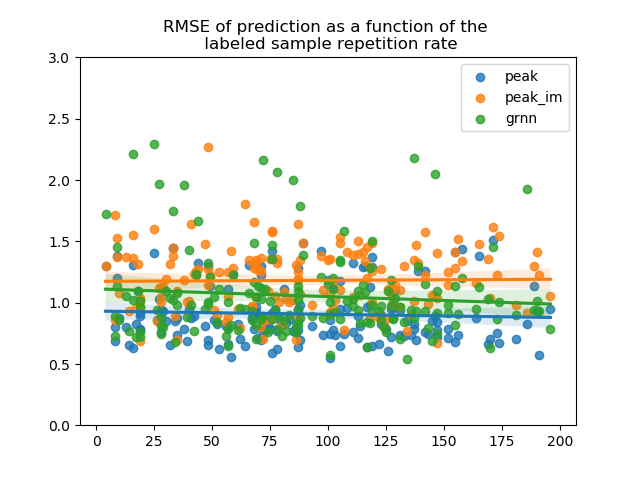
\includegraphics[width=0.4\linewidth]{img/RMSE_krep}
	\caption{Dependency of source position prediction (using our algorithm and two baseline algorithms) RMSE and the rate of labeled training sample reintroduction; linear regression model showed in solid line}
	\label{fig:rmsekrep}
\end{figure}

\begin{figure}[h!]
	\centering
	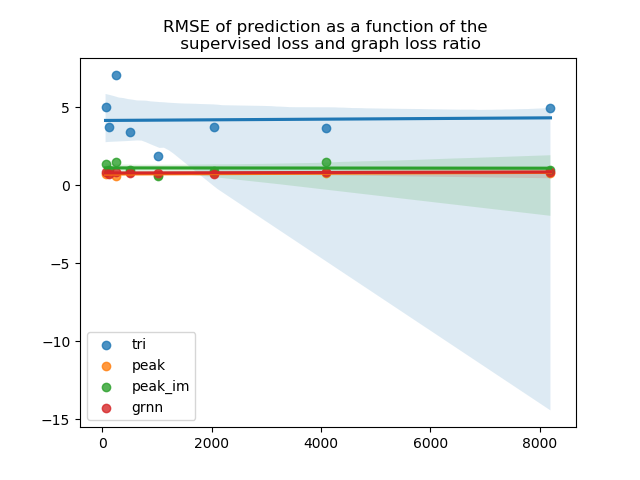
\includegraphics[width=0.4\linewidth]{img/rmse_batch_size}
	\caption{Dependency of source position prediction (using our algorithm and two baseline algorithms) RMSE and the batch size used in \grnn{} training; linear regression model showed in solid line}
	\label{fig:rmsebatchsize}
\end{figure}



%%%%%%%%%%%%%%%%%%%%%%%%%%%%%%%%%%%%%%%%%%
\subsection{Subsection}
\unskip
\subsubsection{Subsubsection}

Bulleted lists look like this:
\begin{itemize}[leftmargin=*,labelsep=5.8mm]
\item	First bullet
\item	Second bullet
\item	Third bullet
\end{itemize}

Numbered lists can be added as follows:
\begin{enumerate}[leftmargin=*,labelsep=4.9mm]
\item	First item 
\item	Second item
\item	Third item
\end{enumerate}

The text continues here.

\subsection{Figures, Tables and Schemes}

All figures and tables should be cited in the main text as Figure 1, Table 1, etc.

\begin{figure}[H]
\centering

\includegraphics[width=2 cm]{Definitions/logo-mdpi}
\caption{This is a figure, Schemes follow the same formatting. If there are multiple panels, they should be listed as: (\textbf{a}) Description of what is contained in the first panel. (\textbf{b}) Description of what is contained in the second panel. Figures should be placed in the main text near to the first time they are cited. A caption on a single line should be centered.}
\end{figure}   
 
Text

Text

\begin{table}[H]
\caption{This is a table caption. Tables should be placed in the main text near to the first time they are cited.}
\centering
%% \tablesize{} %% You can specify the fontsize here, e.g., \tablesize{\footnotesize}. If commented out \small will be used.
\begin{tabular}{ccc}
\toprule
\textbf{Title 1}	& \textbf{Title 2}	& \textbf{Title 3}\\
\midrule
entry 1		& data			& data\\
entry 2		& data			& data\\
\bottomrule
\end{tabular}
\end{table}

Text

Text

%\begin{listing}[H]
%\caption{Title of the listing}
%\rule{\textwidth}{1pt}
%\raggedright Text of the listing. In font size footnotesize, small, or normalsize. Preferred format: left aligned and single spaced. Preferred border format: top border line and bottom border line.
%\rule{\textwidth}{1pt}
%\end{listing}


\subsection{Formatting of Mathematical Components}

This is an example of an equation:

\begin{equation}
a + b = c
\end{equation}
%% If the documentclass option "submit" is chosen, please insert a blank line before and after any math environment (equation and eqnarray environments). This ensures correct linenumbering. The blank line should be removed when the documentclass option is changed to "accept" because the text following an equation should not be a new paragraph. 

Please punctuate equations as regular text. Theorem-type environments (including propositions, lemmas, corollaries etc.) can be formatted as follows:
%% Example of a theorem:
\begin{Theorem}
Example text of a theorem.
\end{Theorem}

The text continues here. Proofs must be formatted as follows:

%% Example of a proof:
\begin{proof}[Proof of Theorem 1]
Text of the proof. Note that the phrase `of Theorem 1' is optional if it is clear which theorem is being referred to.
\end{proof}
The text continues here.

%%%%%%%%%%%%%%%%%%%%%%%%%%%%%%%%%%%%%%%%%%
\section{Discussion}

Authors should discuss the results and how they can be interpreted in perspective of previous studies and of the working hypotheses. The findings and their implications should be discussed in the broadest context possible. Future research directions may also be highlighted.

%%%%%%%%%%%%%%%%%%%%%%%%%%%%%%%%%%%%%%%%%%
\section{Materials and Methods}

In this section, we provide a theoretical background for our investigation.

\ann{}-based sound source localization can be performed using various acoustic features that depend on the sound source, either relative to the microphone array(s) or the acoustic enclosure.

It can be assumed, that acoustic features are spatially smooth, that is, features obtained at spatially close source positions are also close in feature space. The relative distance or affinity of the features can be simply estimated by calculating the Euclidean distance between feature vectors. 

It can be assumed, that high dimensional acoustic features lie on a low-dimensional manifold, embedded in a high-dimensional feature space. 
Since the acoustic features are only dependent on the coordinates of the sound source, it is expected that the manifold would represent the spatial relations between the nearby acoustic features. 
We consider that that the affinity matrix of the low-dimensional embeddings of the acoustic manifold represent the \emph{graph} of the acoustic features.

While the obtained embeddings of the acoustic manifold might represent the relative spatial relations between the acoustic features, it is not tied to physical properties and it also might be very non-linear. The translation of embedded space to physical space must be done in a separate step using a nonlinear regression method. 

When \ann{} is utilized to obtain the sound source position via regression using acoustic features, it might be expected that the predictions of the \ann{} would also exhibit spatial smoothness. Feature manifold could be used during the training of the \ann{} to ensure that the \ann{} learns the relation between the acoustic features and the source positions while also retaining the spatial smoothness.
This spatial smoothness as well as the awareness of the relative spatial positions of the acoustic features is especially important when a semi-supervised learning strategy is involved. Using a training dataset that contains both labeled and unlabeled samples, knowledge of the relative distances between unlabeled and labeled samples might help to train the regressor to predict source locations for the unlabeled samples based on their manifold distance to the labeled features.


Our method is comprised of two stages.
\begin{enumerate}
	\item The low-dimensional embedding of an acoustic feature manifold is obtained from a combined dataset of labeled and unlabeled samples. This manifold represents relative distances between acoustic feature in a low-dimensional embedded space.
	\item A neural network is trained on the combined dataset, using a loss function that consist  of a supervised loss (calculated only for labeled samples) and a graph loss (calculated for all samples, considering $ k $ nearest neighbors). Supervised loss ensures that the regressor is able to learn accurate relations between the acoustic features and the source positions. Graph loss ensures that the source position predictions remain spatially smooth.
\end{enumerate}

Considering that the combined dataset consist of relatively low number of labeled samples and vast amounts of unlabeled samples, the supervised loss acts as a mean to ``straighten'' the manifold while the graph loss is used to infer the labels for the unlabeled samples based on their distance in feature (or embedded) space to the labeled samples.


\subsection{Acoustic Features}
We have considered several types of acoustic features, that are discussed further.

\subsubsection{Time Difference of Arrival}
Time Difference of Arrival (TDoA) is a trivial acoustic feature, that can be estimated using GCC-PHAT. Knowing the TDoA for several non-colinear (or non-parallel?) microphone pairs, it is possible to estimate the position of the sound source using triangulation (trilateration).

While this would be a simple and straightforward method, the accurate TDoA estimation becomes very tricky in reverberant or noisy environments. Moreover, the TDoA contains only very little information about the distance between the sound source and the microphone pair (just one value per pair). For a microphone array with 4 elements, that's only 6 values. TDoA does not explicitly contain any information about the structure of reflections withing the enclosure, nor the geometry or acoustic properties of the enclosure; it only depends on the relative source position with respect to the microphone array(s).

\subsubsection{Room Impulse Response and Room Transfer Function}
It is assumed that high-dimensional acoustic features, such as room impulse response (RIR) or room transfer function (RTF) contain a unique fingerprint of sound source and microphone positions within an enclosure. This is because the structure of room reflections is unique for every source position and every microphone position (theoretically, there might be some cases when same RIR is obtained for more than one combination of microphone and sound source positions, but this is probably possible in ideal room, which exhibit point symmetry around the center of the room; in real rooms this is impossible; also the microphones must be also placed symmetrically in the enclosure for this effect to occur).

While the RIRs and RTFs contain enough information to uniquely determine the position of the source within an enclosure, in practice it is impossible to obtain neither RIR nor RTF without knowing the positions of the sound source and the microphone within the room beforehand.

\subsubsection{Steered Response Power}
Steered Response Power (SRP) and SRP with Phase Transform (\srpphat{}) vectors can be considered the middle ground between the trivial acoustic features like TDoA and ideal features, like RIR or RTF. 
\srpphat{} are obtainable in real world, are relatively high-dimensional and contain information about sound reflections within the room.

\subsubsection{Properties of acoustic features}
The most important property of all acoustic features in this investigation is the spatial smoothness of feature space. In other words, acoustic features are similar to each other for sound source positions that are close together.

In our investigation, we use the \srpphat{} spatial vectors as acoustic features.

\subsection{Acoustic feature acquisition}
Acoustic features were obtained within an acoustic enclosure using a single sound source, $ z $ coordinate was fixed at height \hsrc{}. \Narr{} circular microphone arrays were used for acoustic signal acquisition, each with \Nmic{} microphone elements and radius \rarr{}.
Planes of the microphone arrays were parallel to the ground (normals of the circles coincided with the $ z $ axis of the enclosure).
The both arrays were held at a fixed height \harr{}.
Signals of the microphones are recorded at sampling frequency \fs{} and resolution \resolution{}.


\subsubsection{Unlabeled dataset}
The unlabeled dataset may be obtained from an array audio recording where the sound source is slowly moving inside the acoustic enclosure. The maximal speed of the sound source movement $ \speed_{\src\max} $ should be lower than the maximum expected localization error distance $ \error_{\max} $ per frame duration $ \framedur $:
\begin{equation}\label{eq:unlabeled_src_max_speed}
\speed_{\src\max}  = \frac{\error_{\max}}{\framedur}
\end{equation} 
\subsubsection{Labeled dataset}
The labeled dataset may be obtained from an array audio recordings where the sound source is stationed at a known position $ \spos_{\sposidx} $ within the acoustic enclosure and is producing signal (speech or noise) for a period of \labeledsourceduration{} seconds. A collection of $ \sposidx \in \numel_{\spos} $ recordings at fixed source positions may be obtained.

\subsection{Audio signal framing}

Audio signals obtained from the microphone arrays are split into frames of duration \framedur{} seconds to obtain \Nframes{} frames. For each audio frame $ \frameidx{} \in \Nframes{} $ and for each microphone array $ \arrayidx{} \in \Narr $, a time-frequency representation is calculated with \NFFT{} FFT points and $ \numel_{\mathrm{hop}} $ \todo{kaip tinkamai aprasyti FFT parametrus?} an \srpphat{} spatial spectrum \SRPspectrum{} is obtained. 
\todo{Describe the \srpphat{} acquisition}
\srpphat{} spectra of all arrays are then concatenated per frame to obtain the acoustic feature.

If the audio recording has an associated location label (known coordinates), a frame is assigned the position label \sposlabel{}.

\subsection{Acoustic features selection (thresholding)}

It is considered that the sound source might not be active a all times, and that the signal is non-stationary (in case of speech signal, it might be considered quasi-stationary for frames that contain only one phoneme or a part of a phoneme\todo{cite}). Thus, in case of an audio frame where the source is not active, the \doa{} of a sound source can not be determined, and the acoustic feature is considered to contain only noise. Such frames are to be discarded. For the selection of the audio frames in which the acoustic feature is usable, a thresholding algorithm was used. For each of the frame, a metric 
$ \thrmetric{}_{\arrayidx,\frameidx} $ 
was calculated for and compared to the scaled mean \todo{scaled mean?} of the metric of all obtained frames 
$ \coefficient_\thrmetric \sum_{\frameidx\in\Nframes} \thrmetric{}_{\frameidx}  $, 
where $ \coefficient_\thrmetric $ is the scaling coefficient used to control the threshold value.
The metric used to evaluate the fitness of the acoustic feature of the particular audio frame are: 
\begin{enumerate}
	\item Root-mean-square \todo{maybe that's energy of a frame?} value of the \srpphat{} spectrum, $ \thrmetric_{\rms,\arrayidx,\frameidx} $\todo{kaip prasyti formule SRP spektrui? ten viena dimensija yra kampas - integralas ar suma pagal kampa?}.
	\item Crest factor of the \srpphat{} spectrum, $ \thrmetric_{\cf,\arrayidx,\frameidx} $.
\end{enumerate}


\subsubsection{Training/testing dataset split}
The labeled dataset is split into training and testing subsets by randomly selecting samples from  $ \numel_{\test} $ source positions for training and the rest of the source positions $ \numel_{\train} = \numel_\spos - \numel_\test $ for testing from the entire set of labeled source positions.
Following operations are performed separately for training ant testing labeled datasets.

\subsection{Acoustic manifold embedding learning}

Manifold embedding can be learned using a Nonlinear Dimensionality Reduction (NLDR) algorithm, such as isometric mapping (\isomap{}), t-distributed stochastic neighbor embedding (t-SNE) or localli linear embedding (LLE). 


\subsubsection{\isomap{} embedding}
\srpphat{} features from both labeled and unlabeled training datasets are embedded into \Demb-dimensional embedded space using \isomap{}, with \kemb{} nearest neighbors considered. 
In the resulting embedding, \srpphat{} features are grouped by similarity, while at the same time preserving the spatial structure of the high-dimensional (?) space
%\mpar{Is it really the spatial structure of the high-dimensional space?} (see \figurename{}

\subsection{Graph dataset}

\subsubsection{Dataset preprocessing}
The combined dataset for training the neural network is comprised of two datasets: $ \numel_{\unlabeled} $ acoustic feature samples without source position labels (the unlabeled dataset) and $ \numel_{\labeled} $ acoustic feature samples with source position labels (the labeled training dataset). Each sample in the combined dataset also has a corresponding \isomap{} embedding.
In order to train the \grnn{} with graph regularization, the dataset must be preprocessed: for each sample, regardless of whether it is a labeled or an unlabeled sample, alongside the main feature, neighbor features and their weights must be introduced. This is done by first determining the \gnbrs{} nearest neighbors of a particular sample in the embedded feature space and then appending those features as well as their weight coefficients to the training sample.

\subsubsection{Affinity matrix calculation}
In the embedded space, Euclidean distances are calculated between every feature. The distances between each data sample constitute the distance matrix \distancematrix, which is in turn used to calculate the affinity matrix.
Affinity matrix \affinitymatrix{} is calculated by subtracting \distancematrix{} from 1: $ \affinitymatrix = 1 - \distancematrix $. The distance matrix contains the Euclidean distances between each sample in the low dimensional embedded space:

\begin{align}
	\mathbf{D} &= (d_{ij});\\
	d_{ij} &= \lVert \mathbf{p}_{i}-\mathbf{p}_{j} \rVert _{2}^{2}
\end{align}
here $ \mathbf{p}_{i} = (\alpha_i, \beta_i) $ is the point coordinate vector in the embedded space (in case of $ N_{\mathrm{ISO}} = 2 $), $ \alpha $ and $ \beta $ are the Cartesian coordinates in the embedded space.

Neighbor weights are inversely proportional to the Euclidean distances between the main feature and the neighbor features in the low-dimensional embedded space.

\subsubsection{Neighbor samples and neighbor sample weights}
For the training of the GRNN, each training sample must contain the main \srpphat{} feature and \gnbrs{} neighbor \srpphat{} features (used for calculating the graph loss). Additionally, each neighbor feature is associated with its weight \nbrweigth{}, which is the corresponding element in the affinity matrix.
To obtain the \gnbrs{} neighbors of each sample, each row of the affinity matrix is thresholded so that only the \gnbrs{} highest-valued elements remain their value, while other row elements are set to zero.
The dataset is then expanded so that each sample now has associated neighbor \srpphat{} features (indices of which are the non-zero elements in the rows of the affinity matrix). 


\subsubsection{Labeled/unlabeled sample marking}
For the training dataset, a flag $ m $ denoting wether the sample is labeled or unlabeled is introduced. This flag holds value of either ``True'' of ``False'' (1 or 0). Content of this field is interpreted by the GRNN during the calculation of the loss function. Effectively, the supervised loss component is multiplied by the flag. In case of an unlabeled sample, the supervised loss is ignored, and only the graph loss is considered. In real-world scenario, GRNN expects all fields, including the target feature (the label, the coordinates of the source) to be passed during training. In case of the unlabeled sample (whether during the training phase or during the prediction phase), the supervised loss is not calculated, the label is ignored, and thus it can be set to random values or to zero. 

\subsubsection{Labeled samples repetition}
We wish to train the GRNN using as few as possible labeled samples. It was found that the network is trained more effectively when the labeled samples are introduced more times (more often) than the unlabeled samples. It might be called ``dataset balancing'' \cite{}. 
Labeled samples (those with $ m =  1 $) are repeated $ N_R $ times ($ N_R \in \{1,\dots,199\}$) and appended to the training data subset.

\subsection{Graph-Regularized Neural Network}

In our proposition, a neural network that is trained considering not only the labeled samples, but also neighboring labeled and unlabeled samples.

\subsubsection{Neural network}

Any neural network can be converted to graph-regularized neural network (\grnn) by introducing additional inputs for neighboring features as well as modifying the loss function to accommodate the graph loss.

A general architecture (one of possibilities) of a \grnn model is provided in \figurename{} \ref{fig:networktraining}. In this figure, dotted lines encompasses the input vectors. Dahsed lines inside the GRNN block denote prediction (a forward pass). The loss function is given by $ L = m(\hat{y}_0-y) + \sum_{i \in k_g}a_i(\hat{y}_0 - \hat{y}_1) $. The loss function is discussed further in more detail.

\begin{figure}
	\centering
	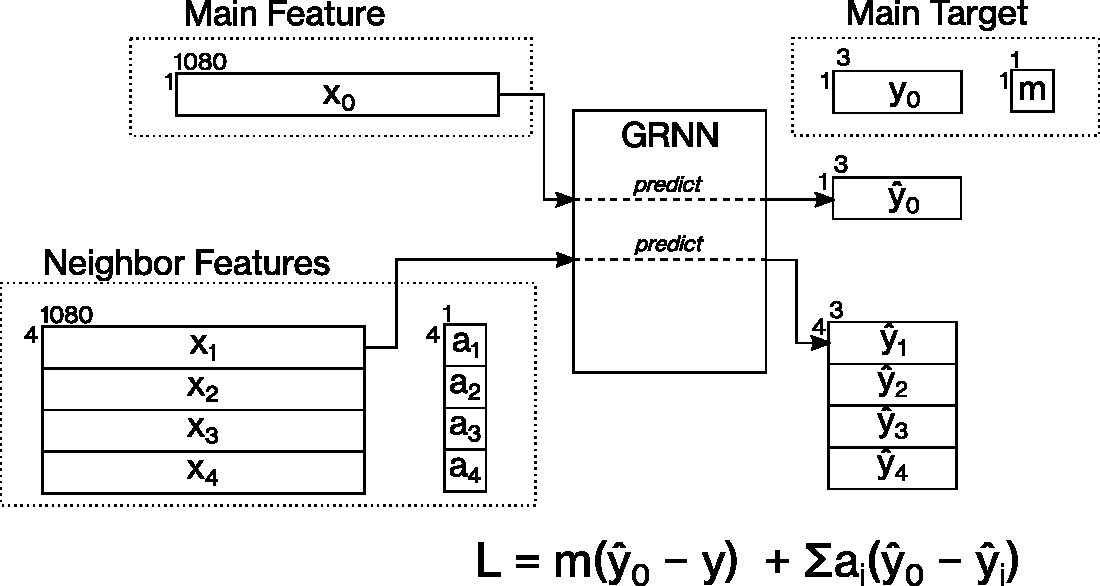
\includegraphics[width=0.5\linewidth]{img/network_training}
	\caption{General architecture of a graph regularized neural network (considering 4 neighbor features). $ x_0 $ is the main input feature, $ x_{1..4} $ are neighbor input features, $ a_{1..4} $ are corresponding neighbor input feature weights, $ y_0 $ is the target feature, $ m $ is the labeled/unlabeled flag, $ \hat{y}_0 $ is the label prediction for main input feature, $ \hat{y}_{1..4} $ are the label predictions for the neighbor input features}
	\label{fig:networktraining}
\end{figure}


\subsubsection{Architecture}
Apart from the introduction of additional inputs (neighbor features, weights and flags), the actual neural network is just a multilayer perceptron. During prediction phase, only the main input contributes to the prediction.

In this experiment, a simple multilayer perceptron architecture was used. 
It contained these layers:
\begin{enumerate}
	\item A 1080-dimensional input layer (to accept a concatenated \srpphat{} feature using $ N_M = 3 $ microphone arrays, each covering \ang{360} azimuth with \ang{1} resolution).
	\item A fully-connected layer with 10 units and linear activations.
	\item A fully-connected layer with 31 units and ReLU activations.
	\item A 3-dimensional output layer with linear activations.
\end{enumerate}

This architecture was the found during previously performed hyperparameter optimization.

%Network architectures that were  used for the experimentation are presented in \tablename{} \ref{table:archs}. The first three architectures were determined during a network architecture optimization process. The last two are the variations of the 3rd architecture.
%
%\begin{table}\footnotesize\setlength{\tabcolsep}{0.3em}
%	\caption{Network achitectures used for the experimentation}\label{table:archs}
%	\begin{tabular}{P{1.4cm}|P{0.6cm}|P{1.4cm}|P{0.6cm}|P{1.4cm}|P{0.6cm}|P{1.4cm}|P{0.6cm}|P{1.4cm}|P{0.6cm}|P{1.4cm}}
%		\toprule
%       & \multicolumn{2}{c}{1st layer} & \multicolumn{2}{c}{2nd layer} & \multicolumn{2}{c}{3rd layer} & \multicolumn{2}{c}{4th layer} & \multicolumn{2}{c}{5th layer} \\
%		\cmidrule(rl){2-3}\cmidrule(rl){4-5}\cmidrule(rl){6-7}\cmidrule(rl){8-9}\cmidrule(rl){10-11}
%		Arch. & N. of units & Activation      & N. of units & Activation      & N. of units & Activation      & N. of units & Activation      & N. of units & Activation      \\ \midrule
%		1                                                                                                    & 14          & linear          & 2           & sigmoid         & 24          & tanh            & 33          & sigmoid         & 50          & linear          \\ \midrule
%		2                                                                                                    & 4           & linear          & 32          & sigmoid         & 23          & tanh            & 54          & sigmoid         & 37          & linear          \\ \midrule
%		3                                                                                                    & 10          & linear          & 31          & ReLU            &             &                 &             &                 &             &                 \\ \midrule
%		4                                                                                                    & 10          & linear          & 15          & ReLU            & 15          & ReLU            &             &                 &             &                 \\ \midrule
%		5                                                                                                    & 10          & linear          & 15          & ReLU            & 15          & ReLU            & 15          & ReLU            & 15          & ReLU            \\ \bottomrule
%	\end{tabular}
%\end{table} 

\subsubsection{Loss function}

Nearby source positions produce similar acoustic features. Therefore, the predicted source positions for the nearby acoustic features should also be similar
If they are similar, the graph loss is small. If they are not similar, we need to penalize the predictor with a large graph loss

The loss function used for the GRNN training is comprised of two parts: the supervised loss (the difference between the ground truth label and the predicted label) and the graph loss (the difference bewteen the main input feature label prediction and the weighted sum of neighbor input features label predictions). It can be expressed as 
\begin{equation}\label{eq:grnn_loss_function}
	L = \mu m \sum_{i \in N_{b}} (\hat{y}_i - y_i)^2  + (1-\mu m) \sum_{i \in N_{b}} \sum_{j \in k_g} a_{ij} (\hat{y}_i-\hat{y}_j)^2
\end{equation}
here $ N_b $ -- number of samples in one training batch, $ k_g $ -- size of the neighborhood, $ a_{ij} $ is the neighbor weight, equal to the corresponding element in the affinity matrix.


\subsection{Experimental setup}
We have evaluated the performance of our proposed method using a \realworld{} microphone array audio dataset with speech signal as the sound source, which was recorded in a particular acoustic enclosure.

\subsubsection{Enclosure}
All audio data used for the experimentation was collected in an irregular shaped room with the side dimensions of \SI{4.902}{\m} in $ x $ axis, \SI{5.361}{\m} in $ y $ axis and \SI{3.75}{\m} in $ z $ axis. The geometry of the enclosure is presented in \figurename{} \ref{fig:room_src_pos}. 

\begin{figure}[h!]
	\centering
	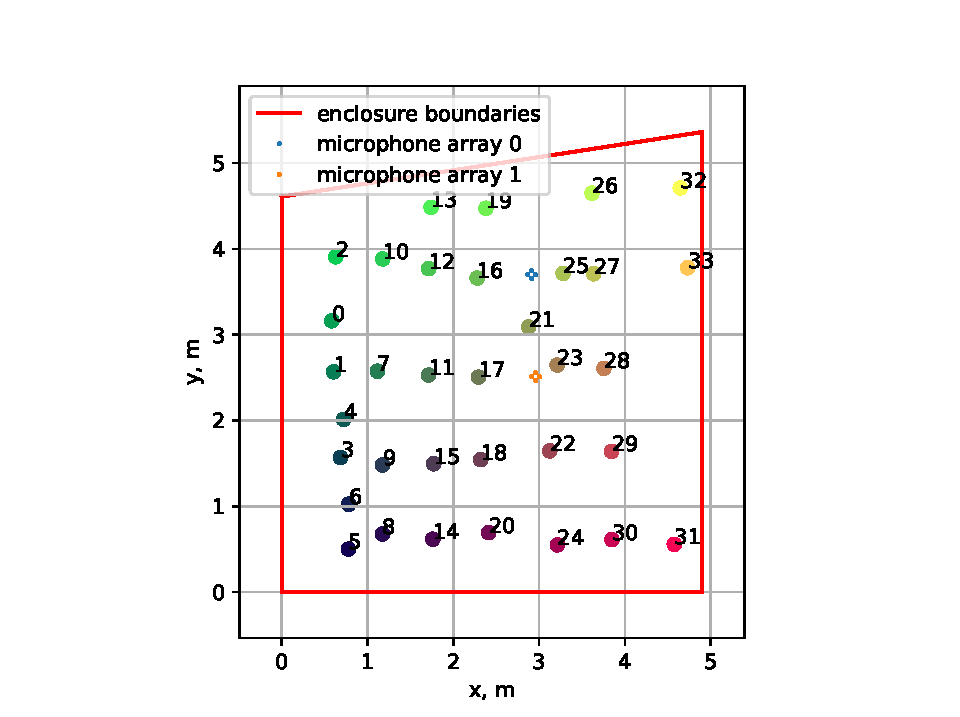
\includegraphics[scale=0.7]{img/room_src_pos.pdf}
	\caption{The geometry of the acoustic enclosure used for \realworld{} dataset collection and labeled sound source positions; height of the enclosure was \SI{3.75}{\m}}\label{fig:room_src_pos}
\end{figure}

\subsubsection{Sound source}
\paragraph{Source signal}
The signal of the sound source was a \SI{1}{\minute} excerpt from the AMI Corpus \cite{carlettaAMIMeetingCorpus2006}, the mix of close-talking microphone signals, containing male and female speech samples.

Sound source signal was reproduced using a compact battery powered loudspeaker that was mounted on an adjustable height stand.

\paragraph{Source positions}
A set of 34 array audio recordings was obtained with the sound source held stationary for \SI{1}{\minute} in one of 34 positions within the enclosure. The coordinates of the sound source were measured using a handheld laser distance measurement tool with accuracy of \SI{1}{\mm}. The locations of the known source positions are presented in \figurename{} \ref{fig:room_src_pos} as colored circles. The values of the red, green and blue components of each circle color are proportional to the $ x_{\src} $, $ y_{\src} $ and $ z_{\src} $ coordinates of the sound source position.
The vertical coordinate, $ z_{\src} = \SI{1.9}{\m} $, was constant for all source positions.

\subsubsection{Unlabeled audio dataset}
The unlabeled audio dataset was collected using the same microphone array setup and the same audio source and signal. The loudspeaker was moved manually at a reasonably constant speed of approximately \SI{0.1}{\m\per\s}, scanning the entire floor area of the enclosure \todo[inline]{by moving along $ y $ axis and then along $ y $ axis -- kaip aprašyti?}. The vertical coordinate of the sound source, $ z = \SI{1.9}{\m} $, was held constant during the entire collection of the unlabeled dataset. 
The total duration of the recording was \SI{511}{\s} \todo{SMF3; SMF4 was 40 minutes long; unused}.

\subsubsection{Microphone arrays}
In our experimentation we have used $ \numel_{\arr} = 2 $ radial microphone arrays with radius $ \radius_{\arr} = \SI{0.045}{\m} $, each consisting of $ \numel_{\mic} = 4 $ microphone elements spaced at equal angles $ \phi_{\mic} = \ang{90} $. The centers of the microphone arrays were placed at coordinates $ \mathbf{M}_{C,1}^{(x,y,z)} = [2.913, 3.699, 1.313]~\si{\m} $\todo{kaip tinkamai uzrasyti koordinaciu rinkini?} and $ \mathbf{M}_{C,2}^{(x,y,z)} = [2.960, 2.512, 1.309]~\si{\m} $.
%    mac = np.array([[2.913, 3.699, 1.313],
%[2.960, 2.512, 1.309]])

First element of each array was oriented towards the positive $ x $ axis with respect to the microphone array center (the rotation of the elements of the microphone array relative to the $ x $ axis was \ang{0}). 

\subsubsection{Acoustic feature acquisition}

Audio signals obtained from the microphone arrays were split into frames with the duration of \SI{0.05}{\s}. This frame duration was chosen so that every audio frame would contain only one speech phoneme.

For each audio frame and for each array, a \srpphat{} spatial spectrum with 360 elements, covering \doa{} of \ang{360} (1 degree resolution) was calculated using \pra{} \python{} implementation \cite{scheiblerr.etal.PyroomacousticsPythonPackage2017} of a method presented in \cite{dibiaseHighaccuracyLowlatencyTechnique2000}. During \srpphat{} spectra calculation, $ \NFFT{} = 512 $ FFT points were used, with \SI{50}{\percent} overlap, for the STFT snapshot calculation. For each frame, \srpphat{} spectra were concatenated to produce a single 720-dimensional acoustic feature.

\subsubsection{Acoustic feature selection}
To select 

\subsubsection{Acoustic feature manifold learning}
Acoustic feature manifold embeddings were found using \isomap{} NLDR algorithm, implemented in \cite{pedregosaScikitlearnMachineLearning2011}.
We have chosen to embed the manifold into 2-dimensional embedded space, since in our experimentation, the only the $ x $ and $ y $ coordinate of the sound source was changing, thus, the acoustic feature are expected to rely only on two variables.
The number of nearest neighbors considered for each sample was selected in the range $ \nneighbors = 2^n; n \in [0,1,\dots,6] $.
The same settings were used for both unlabeled and labeled audio dataset. The acoustic manifold was first learned on unlabeled dataset and then the labeled dataset was transformed into low-dimensional embedded space using the already learned manifold.\todo{patikrinti, ar cia logiskai parastya}

\begin{figure}
	\centering
	\includegraphics[width=0.5\linewidth]{example-image-a}
	\caption{\isomap{} embeddings of acoustic features for unlabeled audio signal, obtained using $ \framedur = \SI{0.05}{\s} $}
	\label{fig:example-image-a}
\end{figure}

\subsubsection{Dataset construction}



%%%%%%%%%%%%%%%%%%%%%%%%%%%%%%%%%%%%%%%%%%
\section{Conclusions}

This section is not mandatory, but can be added to the manuscript if the discussion is unusually long or complex.

%%%%%%%%%%%%%%%%%%%%%%%%%%%%%%%%%%%%%%%%%%
\section{Patents}
This section is not mandatory, but may be added if there are patents resulting from the work reported in this manuscript.

%%%%%%%%%%%%%%%%%%%%%%%%%%%%%%%%%%%%%%%%%%
\vspace{6pt} 

%%%%%%%%%%%%%%%%%%%%%%%%%%%%%%%%%%%%%%%%%%
%% optional
%\supplementary{The following are available online at \linksupplementary{s1}, Figure S1: title, Table S1: title, Video S1: title.}

% Only for the journal Methods and Protocols:
% If you wish to submit a video article, please do so with any other supplementary material.
% \supplementary{The following are available at \linksupplementary{s1}, Figure S1: title, Table S1: title, Video S1: title. A supporting video article is available at doi: link.}

%%%%%%%%%%%%%%%%%%%%%%%%%%%%%%%%%%%%%%%%%%
\authorcontributions{For research articles with several authors, a short paragraph specifying their individual contributions must be provided. The following statements should be used ``Conceptualization, X.X. and Y.Y.; methodology, X.X.; software, X.X.; validation, X.X., Y.Y. and Z.Z.; formal analysis, X.X.; investigation, X.X.; resources, X.X.; data curation, X.X.; writing--original draft preparation, X.X.; writing--review and editing, X.X.; visualization, X.X.; supervision, X.X.; project administration, X.X.; funding acquisition, Y.Y. All authors have read and agreed to the published version of the manuscript.'', please turn to the  \href{http://img.mdpi.org/data/contributor-role-instruction.pdf}{CRediT taxonomy} for the term explanation. Authorship must be limited to those who have contributed substantially to the work reported.}

%%%%%%%%%%%%%%%%%%%%%%%%%%%%%%%%%%%%%%%%%%
\funding{Please add: ``This research received no external funding'' or ``This research was funded by NAME OF FUNDER grant number XXX.'' and  and ``The APC was funded by XXX''. Check carefully that the details given are accurate and use the standard spelling of funding agency names at \url{https://search.crossref.org/funding}, any errors may affect your future funding.}

%%%%%%%%%%%%%%%%%%%%%%%%%%%%%%%%%%%%%%%%%%
\acknowledgments{In this section you can acknowledge any support given which is not covered by the author contribution or funding sections. This may include administrative and technical support, or donations in kind (e.g., materials used for experiments).}

%%%%%%%%%%%%%%%%%%%%%%%%%%%%%%%%%%%%%%%%%%
\conflictsofinterest{Declare conflicts of interest or state ``The authors declare no conflict of interest.'' Authors must identify and declare any personal circumstances or interest that may be perceived as inappropriately influencing the representation or interpretation of reported research results. Any role of the funders in the design of the study; in the collection, analyses or interpretation of data; in the writing of the manuscript, or in the decision to publish the results must be declared in this section. If there is no role, please state ``The funders had no role in the design of the study; in the collection, analyses, or interpretation of data; in the writing of the manuscript, or in the decision to publish the results''.} 

%%%%%%%%%%%%%%%%%%%%%%%%%%%%%%%%%%%%%%%%%%
%% optional
\abbreviations{The following abbreviations are used in this manuscript:\\

\noindent 
\begin{tabular}{@{}ll}
\grnn{} & graph regulzarized neural network \\
SRP & steered response power  \\
PHAT & phase transform \\
\doa{} & direction of arrival \\
RMS & root mean square\\
MSE  & mean squared error \\
MAE   & mean average error \\
RMSE & root mean squared error \\
\isomap{}  & isometric mapping \\
NLDR  & non-linear dimensionality reduction \\
\end{tabular}}

%%%%%%%%%%%%%%%%%%%%%%%%%%%%%%%%%%%%%%%%%%
%% optional
\appendixtitles{no} % Leave argument "no" if all appendix headings stay EMPTY (then no dot is printed after "Appendix A"). If the appendix sections contain a heading then change the argument to "yes".
\appendix
\section{}
\unskip
\subsection{}
The appendix is an optional section that can contain details and data supplemental to the main text. For example, explanations of experimental details that would disrupt the flow of the main text, but nonetheless remain crucial to understanding and reproducing the research shown; figures of replicates for experiments of which representative data is shown in the main text can be added here if brief, or as Supplementary data. Mathematical proofs of results not central to the paper can be added as an appendix.

\section{}
All appendix sections must be cited in the main text. In the appendixes, Figures, Tables, etc. should be labeled starting with `A', e.g., Figure A1, Figure A2, etc. 

%%%%%%%%%%%%%%%%%%%%%%%%%%%%%%%%%%%%%%%%%%
\reftitle{References}

% Please provide either the correct journal abbreviation (e.g. according to the “List of Title Word Abbreviations” http://www.issn.org/services/online-services/access-to-the-ltwa/) or the full name of the journal.
% Citations and References in Supplementary files are permitted provided that they also appear in the reference list here. 

%=====================================
% References, variant A: external bibliography
%=====================================
\externalbibliography{yes}
\bibliography{SS_AS_MDPI_ASC}

%=====================================
% References, variant B: internal bibliography
%=====================================
%\begin{thebibliography}{999}
%% Reference 1
%\bibitem[Author1(year)]{ref-journal}
%Author1, T. The title of the cited article. {\em Journal Abbreviation} {\bf 2008}, {\em 10}, 142--149.
%% Reference 2
%\bibitem[Author2(year)]{ref-book}
%Author2, L. The title of the cited contribution. In {\em The Book Title}; Editor1, F., Editor2, A., Eds.; Publishing House: City, Country, 2007; pp. 32--58.
%\end{thebibliography}

% The following MDPI journals use author-date citation: Arts, Econometrics, Economies, Genealogy, Humanities, IJFS, JRFM, Laws, Religions, Risks, Social Sciences. For those journals, please follow the formatting guidelines on http://www.mdpi.com/authors/references
% To cite two works by the same author: \citeauthor{ref-journal-1a} (\citeyear{ref-journal-1a}, \citeyear{ref-journal-1b}). This produces: Whittaker (1967, 1975)
% To cite two works by the same author with specific pages: \citeauthor{ref-journal-3a} (\citeyear{ref-journal-3a}, p. 328; \citeyear{ref-journal-3b}, p.475). This produces: Wong (1999, p. 328; 2000, p. 475)


%%%%%%%%%%%%%%%%%%%%%%%%%%%%%%%%%%%%%%%%%%
%% optional
\sampleavailability{Samples of the compounds ...... are available from the authors.}

%% for journal Sci
%\reviewreports{\\
%Reviewer 1 comments and authors’ response\\
%Reviewer 2 comments and authors’ response\\
%Reviewer 3 comments and authors’ response
%}

%%%%%%%%%%%%%%%%%%%%%%%%%%%%%%%%%%%%%%%%%%
\end{document}

